\documentclass[11pt,a4paper]{article}

% ============================================================
% PACKAGES
% ============================================================
\usepackage[utf8]{inputenc}
\usepackage[T1]{fontenc}
\usepackage{geometry}
\usepackage{graphicx}
\usepackage{xcolor}
\usepackage{fancyhdr}
\usepackage{titlesec}
\usepackage{booktabs}
\usepackage{array}
\usepackage{tabularx}
\usepackage{hyperref}
\hypersetup{
	hidelinks
}
\usepackage{amsmath}
\usepackage{amssymb}
\usepackage{listings}
\usepackage{tikz}
\usepackage{float}

\geometry{
	a4paper,
	top=2.5cm, bottom=2.5cm,
	left=2.5cm, right=2.5cm,
	headheight=14pt
}

% ============================================================
% COULEURS
% ============================================================
\definecolor{darkblue}{RGB}{0, 51, 102}
\definecolor{darkgray}{RGB}{60, 60, 60}
\definecolor{lightgray}{RGB}{220, 220, 220}
\definecolor{codeblue}{RGB}{30, 90, 150}
\definecolor{akashcolor}{RGB}{0, 100, 150}

% ============================================================
% LISTINGS
% ============================================================
\lstset{
	basicstyle=\ttfamily\small,
	breaklines=true,
	backgroundcolor=\color{lightgray},
	frame=single,
	framerule=0pt,
	numbers=none,
	keywordstyle=\color{codeblue}\bfseries,
	commentstyle=\color{darkgray},
	stringstyle=\color{darkblue},
	showstringspaces=false,
	language=bash,
	morekeywords={hpc, run, run-script}
}

% ============================================================
% STYLES
% ============================================================
\pagestyle{fancy}
\fancyhf{}
\fancyhead[L]{\textbf{HPC Flow}}
\fancyhead[R]{\small White Paper v1.0}
\fancyfoot[C]{\small\thepage}
\renewcommand{\headrulewidth}{0.5pt}

\titleformat{\section}
{\color{darkblue}\Large\bfseries}
{\thesection}{1em}{}[{\vspace{0.2cm}\noindent\color{lightgray}\hrule height 0.5pt}]

\titleformat{\subsection}
{\color{darkblue}\large\bfseries}
{\thesubsection}{0.8em}{}

\titleformat{\subsubsection}
{\color{darkgray}\bfseries}
{\thesubsubsection}{0.8em}{}

\titlespacing{\section}{0pt}{1.2cm}{0.6cm}
\titlespacing{\subsection}{0pt}{0.8cm}{0.4cm}

% ============================================================
% COMMANDES
% ============================================================
\newcommand{\highlight}[1]{\textbf{\color{darkblue}#1}}
\newcommand{\keypoint}[2]{%
	\vspace{0.4cm}
	\noindent\fcolorbox{darkblue}{white}{%
		\begin{minipage}{\dimexpr\linewidth-2\fboxsep-2\fboxrule}
			\vspace{0.1cm}
			{\small\color{darkblue}\textbf{#1}} \quad {\small #2}
			\vspace{0.1cm}
		\end{minipage}%
	}
	\vspace{0.4cm}
}

% ============================================================
% DOCUMENT
% ============================================================
\begin{document}
	
	% ============================================================
	% COUVERTURE
	% ============================================================
	\thispagestyle{empty}
	\vspace*{2cm}
	
	\begin{center}
		{\Huge\color{darkblue}\textbf{HPC Flow}}
		\vspace{0.5cm}
		
		{\Large\color{darkgray}Calcul scientifique simplifié sur infrastructure distribuée}
		\vspace{2cm}
		
		{\large\color{darkgray}\textit{Executer des outils scientifiques sur infrastructure HPC/cloud}}
		
		{\large\color{darkgray}\textit{avec une seule commande}}
		\vspace{3cm}
		
		{\large\color{darkgray}White Paper --- Version 1.0}
		\vspace{0.5cm}
		
		{\small\color{darkgray}Statut : Early Development}
		\vspace{3cm}
		
		{\small\color{darkgray}Akash Network, CLI Open Source}
	\end{center}
	
	\vfill
	
	\noindent\color{darkgray}\small
	\textbf{Acteurs cibles :} CNES, Aix-Marseille Universite, CMA CGM, communautes scientifiques
	
	\newpage
	
	% ============================================================
	% TABLE DES MATIERES
	% ============================================================
	\tableofcontents
	
	\newpage
	
	% ============================================================
	% SECTION 1 : EXECUTIVE SUMMARY
	% ============================================================
	\section{Résumé Exécutif}
	
	\highlight{HPC Flow} est un outil CLI open-source conçu pour simplifier l'exécution de charges de travail scientifiques sur infrastructure distribuée (Akash Network, HPC traditionnels, cloud).
	
	L'objectif : \textit{éliminer la complexité} liée à la containerisation, la configuration d'environnements et le transfert de fichiers.
	
	\subsection{Problème}
	
	Les chercheurs et ingénieurs exécutant des pipelines scientifiques intensifs font face à :
	
	\begin{itemize}
		\item Configuration manuelle de Docker / VMs
		\item Gestion complexe des transferts de fichiers
		\item Apprentissage de multiples outils (AWS CLI, Slurm, etc.)
		\item Administration d'infrastructure consommatrice de temps
		\item Dépendance à un seul fournisseur cloud
	\end{itemize}
	
	\subsection{Solution}
	
	Une interface CLI unique, \highlight{tool-centric}, qui :
	
	\begin{itemize}
		\item Masque la complexité de l'infrastructure
		\item Automatise transfert, provisioning et cleanup
		\item Supporte outils pré-packagés (bioinformatique, géospatial) et scripts custom
		\item Fonctionne sur infrastructure décentralisée (Akash) ou traditionnelle
		\item Reste totalement open-source et extensible
	\end{itemize}
	
	\subsection{Bénéfices pour Chercheurs et Entreprises}
	
	\subsubsection{Pour les chercheurs}
	
	\begin{itemize}
		\item \textbf{Accélération de la recherche} : Moins de temps sur l'infra, plus sur la science. Passer d'une idée à résultats en minutes, pas en semaines.
		\item \textbf{Reproductibilité améliorée} : Environnements isolés et versionnés garantissent que les mêmes résultats sont obtenus partout, par n'importe qui.
		\item \textbf{Collaboration facilitée} : Partager une commande \texttt{hpc-flow run} est plus simple que de documenter une infrastructure entière.
		\item \textbf{Accessibilité} : Aucune expertise DevOps requise. Les scientifiques restent scientifiques.
		\item \textbf{Coûts réduits} : Paiement à l'usage sur Akash Network = \textit{jusqu'à 10x moins cher} qu'AWS ou GCP pour le calcul intensif.
	\end{itemize}
	
	\subsubsection{Pour les entreprises}
	
	\begin{itemize}
		\item \textbf{Time-to-market} : Déployer des pipelines ML/scientifiques sans dépendre d'équipes infra surchargées.
		\item \textbf{Flexibilité} : Utiliser n'importe quel backend (Akash, AWS, HPC local) avec la même commande.
		\item \textbf{Économies d'échelle} : Infrastructure décentralisée = coûts prévisibles et réduction des factures cloud.
		\item \textbf{Propriété intellectuelle protégée} : Calcul distribué sans dépendre d'un seul cloud provider.
		\item \textbf{Gouvernance simplifiée} : Audit et traçabilité intégrés pour conformité réglementaire.
	\end{itemize}
	
	\subsection{Vers une Science Ouverte et Inclusive}
	
	HPC Flow adresse un enjeu critique de l'équité scientifique mondiale : \textit{l'accès au calcul de haute performance}.
	
	\begin{itemize}
		\item \textbf{Démocratisation du calcul} : Chercheurs dans les pays en développement peuvent accéder à infrastructure world-class sans investissement capital massif.
		\item \textbf{Infrastructure décentralisée} : Akash Network distribue le calcul à travers le monde, réduisant dépendances géopolitiques et coûts locaux.
		\item \textbf{Science reproductible} : Code open-source + CLI publique = transparence totale. Chacun peut vérifier, reproduire, améliorer.
		\item \textbf{Communauté mondiale} : Créer liens entre institutions riches et laboratoires ressources limitées. Partage de pipelines scientifiques sans frictions.
		\item \textbf{Impact durable} : Outils gratuits et accessibles = science plus inclusive, résultats plus robustes (peer review global).
	\end{itemize}
	
	\keypoint{CLI Gratuite + Service Managé Payant}{La CLI est open-source et gratuite. Un service web optionnel proposera gestion des jobs, historique, multi-utilisateurs et intégration pour les institutions.}
	
	\newpage

	
	% ============================================================
	% SECTION 2 : ARCHITECTURE TECHNIQUE
	% ============================================================
	\section{Architecture Technique}
	
	\subsection{Vue d'ensemble}
	
	HPC Flow fonctionne selon une architecture simple en trois couches :
	
	\begin{figure}[H]
		\centering
		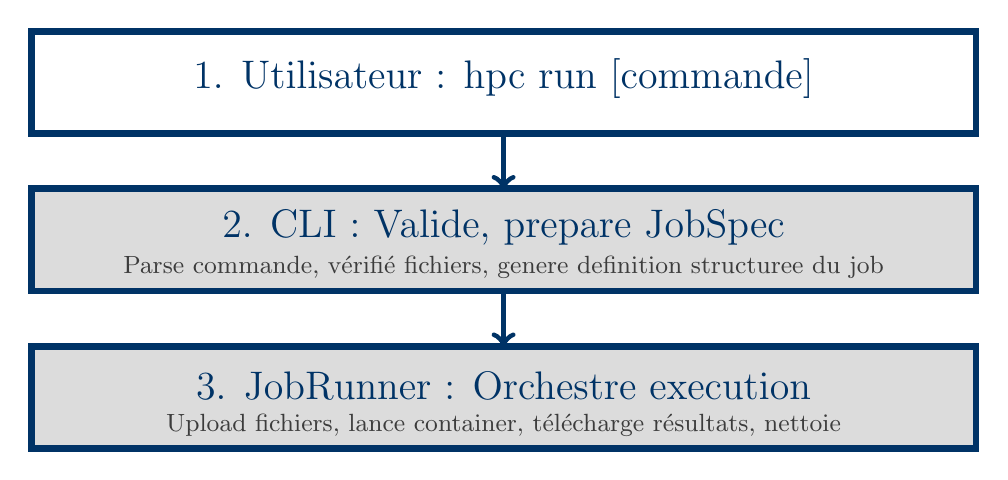
\begin{tikzpicture}[scale=1.0]
			
			% COUCHE 1 : USER
			\draw[darkblue, fill=white, line width=2.5] (-2, 7.5) rectangle (10, 8.8);
			\node[darkblue, font=\bfseries, font=\Large] at (4, 8.2) {1. Utilisateur : hpc run [commande]};
			
			% FLECHE
			\draw[->, line width=2, darkblue] (4, 7.5) -- (4, 6.8);
			
			% COUCHE 2 : CLI
			\draw[darkblue, fill=lightgray, line width=2.5] (-2, 5.5) rectangle (10, 6.8);
			\node[darkblue, font=\bfseries, font=\Large] at (4, 6.3) {2. CLI : Valide, prepare JobSpec};
			\node[darkgray, font=\small] at (4, 5.8) {Parse commande, vérifié fichiers, genere definition structuree du job};
			
			% FLECHE
			\draw[->, line width=2, darkblue] (4, 5.5) -- (4, 4.8);
			
			% COUCHE 3 : JOBRUNNER
			\draw[darkblue, fill=lightgray, line width=2.5] (-2, 3.5) rectangle (10, 4.8);
			\node[darkblue, font=\bfseries, font=\Large] at (4, 4.3) {3. JobRunner : Orchestre execution};
			\node[darkgray, font=\small] at (4, 3.8) {Upload fichiers, lance container, télécharge résultats, nettoie};
			
		\end{tikzpicture}
		\caption{Flux d'exécution simplifié}
	\end{figure}
	
	\subsection{Composants cles}
	
	\subsubsection{1. CLI Layer}
	
	Interface utilisateur minimaliste. L'utilisateur lance une commande simple :
	
	\begin{lstlisting}
		hpc run vsearch \
		--input reads.fasta \
		--id 0.97 \
		--output centroids.fasta \
		--cloud akash
	\end{lstlisting}
	
	La CLI :
	\begin{itemize}
		\item Parse les arguments
		\item Vérifie que le fichier \texttt{reads.fasta} existe localement
		\item Consulte le Tool Registry pour trouver \texttt{vsearch}
		\item Construit une specification de job (JobSpec) en format structurée
	\end{itemize}
	
	\textbf{Pas de Docker, pas de VM, pas de connaissance infrastructure requise.}
	
	\subsubsection{2. Tool Registry}
	
	Catalogue YAML de outils pre-packages. Exemple pour \texttt{vsearch} :
	
	\begin{lstlisting}
		name: vsearch
		version: "2.28.1"
		image: quay.io/biocontainers/vsearch:2.28.1
		parameters:
		- name: input
		flag: --fastx_uniques
		- name: id
		flag: --id
		resources:
		cpu: 4
		memory: 8Gi
	\end{lstlisting}
	
	Chacun peut contribuer de nouveaux outils (bioinformatique, geospatial, etc.).
	
	\subsubsection{3. JobRunner Interface}
	
	Abstraction generique permettant de soutenir différents backends sans changer le code CLI.
	
	\begin{lstlisting}
		interface JobRunner:
		- submit(job) -> job_id
		- status(job_id) -> pending|running|succeeded|failed
		- fetch_results(job_id) -> fichiers_locaux
		- cleanup(job_id)
	\end{lstlisting}
	
	\subsubsection{4. Backend Implementations}
	
	\textbf{Phase 1 (MVP) :} AkashJobRunner
	\begin{itemize}
		\item Upload fichiers d'entrée sur Akash
		\item Crée un deployment Akash avec l'image du tool
		\item Monitore l'execution via logs Akash
		\item Télécharge les résultats
		\item Detruit le deployment
	\end{itemize}
	
	\textbf{Phase 2+ :} Support AWS, GCP, Slurm
	\begin{itemize}
		\item AWSJobRunner : utilise Lambda ou EC2
		\item GCPJobRunner : utilise Cloud Run ou Compute Engine
		\item SlurmJobRunner : intégration HPC traditionnels
	\end{itemize}
	
	\subsubsection{5. Script Execution Custom}
	
	Pour les scientifiques avec pipelines spécifiques :
	
	\begin{lstlisting}
		hpc run-script mon_analyse.py \
		--runtime python:3.11 \
		--input data.csv \
		--output result.html \
		--cloud akash
	\end{lstlisting}
	
	Le script et ses dépendances (\texttt{requirements.txt}) sont uploades et exécutes dans un runtime de base.
	
	\newpage
	
	% ============================================================
	% SECTION 3 : WORKFLOW
	% ============================================================
	\section{Workflow d'Execution}
	
	\subsection{Flux d'une commande hpc run}
	
	\begin{enumerate}
		\item \textbf{Parsing} : CLI interprète la commande et flags
		
		\item \textbf{Validation} : Controle existence fichiers, validite flags, ressources disponibles
		
		\item \textbf{JobSpec construction} : Creation d'une description structurée du job
		
		\item \textbf{Backend selection} : Choix du JobRunner (Akash, AWS, etc.)
		
		\item \textbf{Resource provisioning} : Allocation ressources sur le backend
		
		\item \textbf{File upload} : Transfert fichiers d'entrée vers remote
		
		\item \textbf{Job execution} : Lancement du container avec arguments
		
		\item \textbf{Monitoring} : Polling status, capture logs
		
		\item \textbf{Result download} : Récuperation fichiers output en local
		
		\item \textbf{Cleanup} : Destruction du deployment
	\end{enumerate}
	
	\textbf{Duree totale :} Quelques secondes (provisioning) + temps calcul + quelques secondes (download).
	
	\newpage
	
	% ============================================================
	% SECTION 4 : CAS D'USAGE
	% ============================================================
	\section{Cas d'Usage Cibles}
	
	\subsection{Bioinformatique}
	
	\subsubsection{Analyse sequences (CNES, Universites)}
	
	Chercheurs en biologie evolutive nécessitent clustering de milliers de sequences ADN.
	
	\begin{lstlisting}
		hpc run vsearch \
		--input metagenome_1M_reads.fasta \
		--id 0.97 \
		--threads 16 \
		--output centroids.fasta \
		--cloud akash
	\end{lstlisting}
	
	\textbf{Avantage :} Une commande. Pas d'administration infrastructure.
	
	\subsubsection{BLAST / alignment (Biotech, Universite)}
	
	\begin{lstlisting}
		hpc run blast \
		--query proteins.fasta \
		--db nr \
		--output results.tsv \
		--cloud akash
	\end{lstlisting}
	
	\subsection{Geospatial}
	
	\subsubsection{Traitement rasters DEM (CNES, CMA CGM logistics)}
	
	Calcul de pentes, d'exposition, d'indices de vegetation sur images satellites.
	
	\begin{lstlisting}
		hpc run geoprocess \
		--input dem_region.tif \
		--operation slope \
		--output slope_map.tif \
		--cloud akash
	\end{lstlisting}
	
	\textbf{Cas d'usage CMA CGM :} Optimisation logistique via analyse relief terrain pour planification trajets.
	
	\subsection{Scripts Custom}
	
	\subsubsection{Analyse donnees proprietaires}
	
	Chercheur avec pipeline specifique (combinaison outils maison + libs standard).
	
	\begin{lstlisting}
		hpc run-script analyse_propriete.py \
		--runtime python:3.11 \
		--input data_confidentiel.csv \
		--output rapport.html \
		--cloud akash
	\end{lstlisting}
	
	Fichier requirements.txt est telecharge automatiquement.
	
	\newpage
	
	% ============================================================
	% SECTION 5 : AKASH NETWORK --- PREMIER BACKEND
	% ============================================================
	\section{Akash Network : Premier Backend et Strategie Multi-Cloud}
	
	\subsection{Qu'est-ce qu'Akash Network ?}
	
	Akash Network est une marketplace décentralisée de ressources cloud basée sur la technologie blockchain. Contrairement aux fournisseurs cloud traditionnels (AWS, Google Cloud, Azure), Akash fonctionne en peer-to-peer : les utilisateurs achètent et vendent de la puissance de calcul (CPU, GPU, mémoire) directement auprès de fournisseurs indépendants (nodes), sans intermédiaire centralisé.
	
	Fonctionnement clé :
	
	Les fournisseurs (nodes) proposent leurs ressources inutilisées sur le réseau.
	Les utilisateurs paient avec des tokens AKASH (AKT) pour louer ces ressources (Le but du service managé est d'éliminer cette étape pour l'utilisateur).
	Les deployments sont isolés et sécurisés grâce à des conteneurs Kubernetes natifs.
	Coûts réduits : Jusqu'à 80\% moins chers que les clouds centralisés grâce à l'absence d'intermédiaires.
	Infrastructure ouverte : Pas de lock-in, compatibilité avec les outils standards (Docker, Kubernetes).
	Décentralisé : Pas de dépendance à un seul fournisseur, résilience accrue.
	
	Akash est souvent surnommé le "Airbnb du cloud" car il permet aux propriétaires de matériel de monétiser leurs ressources inutilisées, tout en offrant aux utilisateurs une alternative économique et flexible aux clouds traditionnels.
	
	\subsection{Pourquoi Akash Network ?}
	
	Akash Network est choisi comme \textbf{premier backend} pour HPC Flow pour plusieurs raisons strategiques :
	
	\subsubsection{Avantages distinctifs}
	
	\begin{table}[H]
		\centering
		\small
		\begin{tabularx}{\linewidth}{l | c | c | c}
			\toprule
			\textbf{Critere} & \textbf{Akash} & \textbf{AWS} & \textbf{GCP} \\
			\midrule
			Décentralisé & $\checkmark$ & $\times$ & $\times$ \\
			Prix 60-80\% moins cher & $\checkmark$ & Baseline & $\approx$ AWS \\
			Pas de lock-in fournisseur & $\checkmark$ & $\times$ & $\times$ \\
			Marché ouvert (peer-to-peer) & $\checkmark$ & $\times$ & $\times$ \\
			Facile intégration containers & $\checkmark$ & $\checkmark$ & $\checkmark$ \\
			\bottomrule
		\end{tabularx}
		\caption{Comparaison Akash vs cloud centralisé}
	\end{table}
	
	\paragraph{1. Decentralisation et Souveraineté}
	Akash est une blockchain decentralisée. Aucun acteur unique ne controle l'infrastructure. Ideal pour :
	\begin{itemize}
		\item CNES : pas de dependance geopolitique pour donnees spatiales
		\item CMA CGM : donnees logistiques sensibles non centralisees
		\item Universités : data governance flexible
	\end{itemize}
	
	\paragraph{2. Economies d'echelle}
	Prix \textbf{60-80\% moins chers} que AWS/GCP grace au modele P2P. Les fournisseurs (providers) Akash optimisent leurs couts.
	
	\paragraph{3. Absence de lock-in}
	Architecture multi-backend permet switch vers autre cloud sans changer code utilisateur. Leverage concurrentiel durable.
	
	\paragraph{4. Marche ouvert}
	Providers multiples (node operators) enchérissent pour jobs. Transparence des prix. Pas de tarification captive.
	
	\subsection{Limitations actuelles d'Akash et trajectoire}
	
	\subsubsection{Limitations presentes}
	
	\begin{itemize}
		\item \textbf{Maturite reseau} : Variabilite de disponibilite compute. Certains providers peuvent etre offline.
		\item \textbf{Offre limitee compute} : Moins de GPU haute performance que AWS. Mieux adapte a CPU/GPU standard.
		\item \textbf{Stockage objet} : Pas d'equivalent S3 natif. Fichiers volumineux requierent up/download.
		\item \textbf{Ecosystem outillage} : Outils monitoring et observabilite moins matures que AWS CloudWatch.
		\item \textbf{Support technique} : Communaute emergente, moins de support enterprise.
		\item \textbf{SLA garanties} : Pas de garanties SLA formelles (work in progress).
	\end{itemize}
	
	\subsubsection{Developpements planifies Akash (roadmap 2024-2025)}
	
	Akash Network s'améliore activement :
	
	\begin{itemize}
		\item \textbf{Persistent Volumes} : Stockage persistent sur deployments (Phase actuelle)
		\item \textbf{Upgrade GPU support} : Meilleur support NVIDIA H100, A100
		\item \textbf{Akash Console} : Dashboard web pour managment deployments
		\item \textbf{Akash SLA Guarantees} : SLA formels en 2024-Q4
		\item \textbf{Akash Storage} : Solution stockage decentralisee (similar S3)
		\item \textbf{Improved Provider ecosystem} : Plus de providers, meilleure qualite service
	\end{itemize}
	
	\keypoint{HPC Flow aligne sur evolution Akash}{Au fur et a mesure de l'evolution Akash, HPC Flow herite automatiquement des ameliorations (persistent storage, GPU avances, SLA).}
	
	\newpage
	
	\subsection{Strategie Multi-Cloud et Selection Backend}
	
	\textbf{Vision long-terme} : HPC Flow abstrait l'infrastructure. L'utilisateur choisit backend selon besoin.
	
	\subsubsection{Selection Backend : Par commande}
	
	L'utilisateur specifie backend directement dans la commande :
	
	\begin{lstlisting}
		# Utiliser Akash (par defaut, economique)
		hpc run vsearch --input data.fasta --cloud akash
		
		# Utiliser AWS pour job critique necessite SLA 99.99%
		hpc run blast --input proteins.fasta --cloud aws --instance-type c5.4xlarge
		
		# Utiliser HPC traditionnel pour GPU haute perf
		hpc run deeplearning --input train.tar --cloud slurm --partition gpu
	\end{lstlisting}
	
	\subsubsection{Selection Backend : Par profil utilisateur}
	
	Phase 2 : Configuration persistante dans \texttt{\textasciitilde/.hpc/config.yaml} :
	
	\begin{lstlisting}
		# Profil par defaut
		default_cloud: akash
		
		# Overrides par type de job
		cloud_rules:
		- match:
		tool: blast
		input_size: ">10GB"
		cloud: aws
		
		- match:
		tool: deeplearning
		cloud: aws
		gpu: true
		instance_type: p3.8xlarge
		
		- match:
		runtime: python
		memory_required: ">16Gi"
		cloud: slurm
		partition: gpu
	\end{lstlisting}
	
	Avantages :
	\begin{itemize}
		\item \textbf{Flexibilite} : Scientifique choisit meilleur cloud par cas d'usage
		\item \textbf{Optimisation couts} : Akash par defaut pour jobs standards, AWS pour critiques
		\item \textbf{Pas de re-apprentissage} : Syntaxe CLI reste identique
	\end{itemize}
	
	\subsubsection{Backends planifies}
	
	\textbf{Phase 1 (2024-Q2) :}
	\begin{itemize}
		\item AkashJobRunner (MVP)
	\end{itemize}
	
	\textbf{Phase 2 (2024-Q4) :}
	\begin{itemize}
		\item AWSJobRunner (EC2 + Lambda)
		\item Local Slurm JobRunner (HPC traditionnel)
	\end{itemize}
	
	\textbf{Phase 3 (2025-Q1+) :}
	\begin{itemize}
		\item GCPJobRunner (Compute Engine + Cloud Run)
		\item SecNumCloud JobRunner (infrastructure francaise sovereign)
		\item Azure JobRunner
		\item Kubernetes generic JobRunner (on-prem, managed k8s)
	\end{itemize}
	
	\subsection{Cas d'usage par backend}
	
	\subsubsection{Akash : Jobs scientifiques standards}
	
	\textbf{Ideal pour :}
	\begin{itemize}
		\item Jobs CPU/GPU standards (non-critique)
		\item Workloads bioinformatique (vsearch, BLAST, SAMtools)
		\item Geospatial processing avec GDAL/QGIS
		\item Recherche academique (budget constraints)
		\item Development et experimentation (prototypage)
	\end{itemize}
	
	\textbf{Prix estimatif} (approximations 2026) :
	\begin{itemize}
		\item CPU 4-core, 8GB RAM : \$0.05-0.10 par heure vs \$0.25 AWS
		\item GPU L40 : \$0.30-0.50 par heure vs \$1.00+ AWS
	\end{itemize}
	
	
	\subsubsection{HPC Traditionnel (Slurm) : Institutions}
	
	\textbf{Ideal pour :}
	\begin{itemize}
		\item Universites/Labos avec infrastructure interne
		\item Workloads MPI paralleles massifs
		\item Donnees sensibles on-premise
		\item Integration pipelines HPC existants
	\end{itemize}
	
	\subsubsection{SecNumCloud : Donnees francaises regulees}
	
	\textbf{Ideal pour :}
	\begin{itemize}
		\item CNES : Donnees spatiales classification defense
		\item Entites publiques : Conformite cloud souverain francais
		\item Biotech pharma : Donnees patients confidentielles
		\item Infrastructure 100\% France hebergement garantis
	\end{itemize}
	
	\newpage
	
	% ============================================================
	% SECTION 6 : MODELE ECONOMIQUE
	% ============================================================
	\section{Modele Economique}
	
	\subsection{CLI Open-Source (Gratuit)}
	
	\begin{itemize}
		\item Code source MIT licence
		\item Installation locale : pip install hpc-flow
		\item Utilisation illimitee (couts infra a charge utilisateur)
		\item Contributions communaute bienvenues
	\end{itemize}
	
	\subsection{Service Manage (Payant / SaaS)}
	
	Phase 2-3 : plateforme web optionnelle pour :
	
	\begin{itemize}
		\item \textbf{Gestion multi-utilisateurs} : Teams, projets, quotas
		\item \textbf{Historique et monitoring} : Jobs, logs, duree, couts
		\item \textbf{Dashboard web} : Lancement jobs, suivi, resultats
		\item \textbf{Integration API} : Appels programmatiques
		\item \textbf{Support technique} : SLA garanti
	\end{itemize}
	
	\keypoint{Tarification estimee (Phase 3)}{Modele freemium : gratuit jusqu'a X jobs/mois, puis tarification a l'usage ou abonnement institutional.}
	
	\newpage
	
	% ============================================================
	% SECTION 7 : STATUT & ROADMAP
	% ============================================================
	\section{Statut et Roadmap}
	
	\subsection{Phase 1 --- MVP / POC (En cours)}
	
	\textbf{Objectif :} CLI fonctionnelle + backend Akash + 2-3 outils de demo.
	
	\begin{itemize}
		\item[$\checkmark$] Architecture generique JobRunner
		\item[$\checkmark$] Implementation AkashJobRunner
		\item[$\checkmark$] CLI parsing et JobSpec
		\item[$\checkmark$] Tool registry (vsearch, geoprocess)
		\item[$\checkmark$] File transfer (upload/download)
		\item[$\checkmark$] Script execution (Python)
		\item[\,-] Demonstration POC (bioinformatique + geospatial)
	\end{itemize}
	
	\textbf{Timeline :} 2-3 mois
	
	\subsection{Phase 2 --- Hardening et Multi-Cloud}
	
	\textbf{Objectif :} CLI production-ready, support AWS + Slurm, configuration profile.
	
	\begin{itemize}
		\item[\,-] Outils additionnels (BLAST, SAMtools, GDAL complets)
		\item[\,-] Runtimes script : Bash, R, Julia
		\item[\,-] Job history local (hpc log, hpc history)
		\item[\,-] AWSJobRunner implementation
		\item[\,-] SlurmJobRunner implementation
		\item[\,-] Config file support (\textasciitilde/.hpc/config.yaml)
		\item[\,-] Cloud selection logic
		\item[\,-] Error handling robuste
	\end{itemize}
	
	\textbf{Timeline :} 3-4 mois apres Phase 1
	
	\subsection{Phase 3 --- Managed Layer et Multi-Cloud}
	
	\textbf{Objectif :} SaaS optionnel, support multi-cloud (GCP, SecNumCloud, Azure).
	
	\begin{itemize}
		\item[\,-] Web app / dashboard
		\item[\,-] User et project management
		\item[\,-] GCPJobRunner implementation
		\item[\,-] SecNumCloud integration (partnership)
		\item[\,-] Azure support
		\item[\,-] API REST
		\item[\,-] Pricing engine (cost estimation)
		\item[\,-] Advanced resource prediction
	\end{itemize}
	
	\textbf{Timeline :} 4-6 mois apres Phase 2
	
	\newpage
	
	% ============================================================
	% SECTION 8 : AVANTAGES COMPETITIFS
	% ============================================================
	\section{Avantages Competitifs}
	
	\begin{table}[H]
		\centering
		\small
		\begin{tabularx}{\linewidth}{l | c | c | c}
			\toprule
			\textbf{Critere} & \textbf{HPC Flow} & \textbf{Cloud classique} & \textbf{HPC trad.} \\
			\midrule
			Pas Docker/VM requis & $\checkmark$ & $\times$ & $\times$ \\
			Interface tool-centric & $\checkmark$ & $\times$ & $\times$ \\
			Decentralise / multi-cloud & $\checkmark$ & $\times$ & $\times$ \\
			Transfert fichiers auto & $\checkmark$ & Manuel & Manuel \\
			Cleanup automatique & $\checkmark$ & Manuel & Manuel \\
			Open-source et extensible & $\checkmark$ & $\times$ & Partiel \\
			Economique (pay-as-you-go) & $\checkmark$ & $\checkmark$ & Abonnement \\
			Courbe apprentissage faible & $\checkmark$ & $\times$ & $\times$ \\
			\bottomrule
		\end{tabularx}
		\caption{Positionnement marche}
	\end{table}
	
	\newpage
	
	% ============================================================
	% SECTION 9 : IMPACT POUR LES ACTEURS CIBLES
	% ============================================================
	\section{Impact pour les Acteurs Cibles}
	
	\subsection{CNES (Centre National Etudes Spatiales)}
	
	\begin{itemize}
		\item \textbf{Defi} : Traitement massif de donnees geospatiales (satellites), infrastructure couteuse, souverainete donnees
		\item \textbf{Apport HPC Flow} : Execution pipelines geospatial sur Akash ou SecNumCloud (economies + souverainete), API extensible, pas de lock-in fournisseur
		\item \textbf{Cas d'usage} : Analyse DEM, detection objets, classification satellite
		\item \textbf{Gain economique} : -60\% couts compute vs AWS avec Akash
	\end{itemize}
	
	\subsection{Aix-Marseille Universite}
	
	\begin{itemize}
		\item \textbf{Defi} : Chercheurs heterogenes, pas d'equipe infra dediee, couts cloud eleves
		\item \textbf{Apport HPC Flow} : Outil simple pour tous, auto-heberge ou sur Akash, pas d'administration
		\item \textbf{Cas d'usage} : Bioinformatique, chimie quantique, geospatial, analyses data science
		\item \textbf{Gain} : Democratisation acces HPC, reduction charge IT
	\end{itemize}
	
	\subsection{CMA CGM (Logistique Maritime)}
	
	\begin{itemize}
		\item \textbf{Defi} : Optimisation trajets, predictions, besoin compute on-demand sans over-capacity
		\item \textbf{Apport HPC Flow} : Integration facile dans pipelines data, scaling elastique, couts proportionnels, choix cloud (Akash ou intégration interne)
		\item \textbf{Cas d'usage} : Analyse relief (trajets marins), prédictions météo, optimisation routes
		\item \textbf{Gain} : Flexibilité coûts, pas d'over-provisioning
	\end{itemize}
	
	\subsection{Akash Network}
	
	\begin{itemize}
		\item \textbf{Defi} : Augmenter adoption compute decentralisé, proposer outils hauts niveaux
		\item \textbf{Apport HPC Flow} : Killer app pour scientifiques, abstraire complexite Akash, bootstrap communaute scientifique
		\item \textbf{Synergies} : Co-marketing, intégration Akash API, case studies communs, accélération providers adoption
	\end{itemize}
	
	\newpage
	
	% ============================================================
	% SECTION 10 : RISQUES & MITIGATION
	% ============================================================
	\section{Risques et Mitigation}
	
	\begin{table}[H]
		\centering
		\small
		\begin{tabularx}{\linewidth}{l | p{5.5cm} | p{4cm}}
			\toprule
			\textbf{Risque} & \textbf{Description} & \textbf{Mitigation} \\
			\midrule
			Akash Network immaturité & Variabilité prix, disponibilité compute & Multi-cloud. \\
			Adoption lente & Chercheurs habitués aux outils éxistants & POC public + démos, partenariats institution et entreprise \\
			Fragmentation registry & Trop d'outils, mauvaise maintenance & Governance claire, guidelines, CI/CD, code review \\
			Scaling limite Akash & Bottleneck transfert fichiers volumineux & S3 URLs, streaming, multi-cloud fallback \\
			Support utilisateurs & Demande support technique croissante & SaaS managed Phase 3, docs excellentes, communauté \\
			Compatibilité backends & Divergences syntaxe AWS vs GCP & Abstraction uniforme JobRunner \\
			\bottomrule
		\end{tabularx}
	\end{table}
	
	\newpage
	
	% ============================================================
	% SECTION 11 : CONCLUSION
	% ============================================================
	\section{Conclusion}
	
	\highlight{HPC Flow} adresse un besoin réel et universel : simplifier l'exécution de charges de travail scientifique sans expertise infra, tout en préservant la \textbf{liberté de choix} sur l'infrastructure.
	
	\subsection{Forces cles}
	
	\begin{enumerate}
		\item \textbf{Simplicité} : Une commande pour tout. Pas Docker, pas VM, pas de tracas.
		\item \textbf{Flexibilite} : Open-source, extensible, multi-cloud par architecture.
		\item \textbf{Decentralisation} : Akash Network comme premier backend, autres possibles.
		\item \textbf{Economies} : 60-80\% reduction couts compute vs cloud centralisé (Akash Phase 1).
		\item \textbf{Communaute} : Registry contributif, MIT licence, contributions bienvenues.
		\item \textbf{Modele durable} : CLI gratuite + SaaS optionnel.
		\item \textbf{Multi-cloud} : Jamais enfermé. Eviter lock-in fournisseur.
	\end{enumerate}
	
	\subsection{Prochaines etapes}
	
	\begin{itemize}
		\item Phase 1 : POC fonctionnel Akash (fin Q2 2024)
		\item Partenariats : CNES, Aix-Marseille, Akash Network
		\item Publication + presentation conferences scientifiques (JRES, ADP)
		\item Recrutement contributeurs open-source
		\item Phase 2 : Multi-cloud (AWS, Slurm) fin Q4 2024
	\end{itemize}
	
	\vspace{1cm}
	
	\noindent\fcolorbox{darkblue}{white}{%
		\begin{minipage}{\dimexpr\linewidth-2\fboxsep-2\fboxrule}
			\vspace{0.2cm}
			\small\color{darkblue}\textbf{HPC Flow : rendre le calcul scientifique accessible a tous, avec choix infrastructure et couts optimisés.}
			\vspace{0.2cm}
		\end{minipage}%
	}
	
	\newpage
	
	% ============================================================
	% APPENDIX
	% ============================================================
	\appendix
	
	\section{Glossaire Technique}
	
	\begin{tabularx}{\linewidth}{l X}
		\toprule
		\textbf{Terme} & \textbf{Definition} \\
		\midrule
		\textbf{HPC} & High Performance Computing - Calcul haute performance \\
		\textbf{Akash Network} & Marche decentralise peer-to-peer de ressources computationnelles blockchain \\
		\textbf{CLI} & Command-Line Interface - Interface en ligne de commande \\
		\textbf{JobSpec} & Specification structuree d'un job (outil, args, fichiers, ressources) \\
		\textbf{JobRunner} & Abstraction pour soumettre jobs a un backend (Akash, AWS, Slurm) \\
		\textbf{Registry} & Catalogue de definitions d'outils \\
		\textbf{POC} & Proof of Concept - Validation technique d'un concept \\
		\textbf{YAML} & Format texte lisible pour donnees structurees \\
		\textbf{API} & Application Programming Interface - Interface programmation \\
		\textbf{SLA} & Service Level Agreement - Accord niveau service \\
		\textbf{P2P} & Peer-to-Peer - Architecture distribuée sans intermédiaire central \\
		\textbf{Lock-in} & Dépendance a un seul fournisseur sans moyen d'en changer \\
		\textbf{SecNumCloud} & Référentiel francais cloud souverain, sécurité renforcée \\
		\bottomrule
	\end{tabularx}
	
	\section{References}
	
	\begin{itemize}
		\item GitHub Repository : https://github.com/hdavid-13/hpc-flow
		\item Akash Network : https://akash.network
		\item Akash Roadmap : https://github.com/akash-network/roadmap
		\item Biocontainers : https://biocontainers.pro
		\item SecNumCloud : https://www.ssi.gouv.fr/entreprise/qualifications/
	\end{itemize}
	
	
\end{document}
